\chapter{Methodology}
\label{chapter:Methodology}

The following chapter details the physical setup to develop the measurements that constitute the dataset under study, also present a description of testbench and processing pipeline in which the data flows from the acoustic inputs towards the desire location-orientation output.       

\section{Experiment Design}

The process starts with the data collection under an experimental setup, the data will be curated to eliminate random noise and presented as a time series dataset. The resulting dataset will be used to train and test four neural network pipelines. The predicted location-orientation error is calculated and a multifactor Analysis of Variance (ANOVA) is proposed as the main criteria to evaluate the significant variance of the error of each processing pipeline used to estimate the location and orientation of an object in a room. 
 

\label{section:experiment-design}

\section{Experimental measurement configuration}


The research require the development of a manipulable and fully controllable environment in which the acoustic measurements are going to be performed. A small box type room is the volumetric cubic space used as the experimental container. The container used for the experimental measurements is a cubic box with sides of 1m in length and a volume close to $1m^3$, the concept is show in Figure \ref{mesurementbox} (a), three of its six walls are built from porcelain tiles with a thickness of 
1cm, one wall an the floor are made of solid concrete, while the remaining wall used for observation is made of acrylic with a thickness of 0.5cm. The clear acrylic sheet allows direct observation of the movement mechanism inside the box. Unlike the other walls, which are permanently bonded, this acrylic wall can be removed to provide access to the interior of the measurement box. The movement mechanism inside the box consists of a robotic arm mounted at the center of the floor. The arm has four Degrees Of Freedom (DOF) and is used to move and change the position and orientation of a small cube with 20cm side length attached to its end. The cube is made of plastic, with walls of 2mm thickness. For the measurements, a mono speaker is placed at the center of one wall to generate the acoustic stimulus inside the system. On the opposite wall, four capacitive microphones are positioned 10cm away from each corner, with the purpose of capturing the acoustic response of the measurement box. The implementation of the measurement box was build inside a storage room and is presented in the Figure \ref{mesurementbox} (b).



\begin{figure}[!htb]
        \begin{center}        
            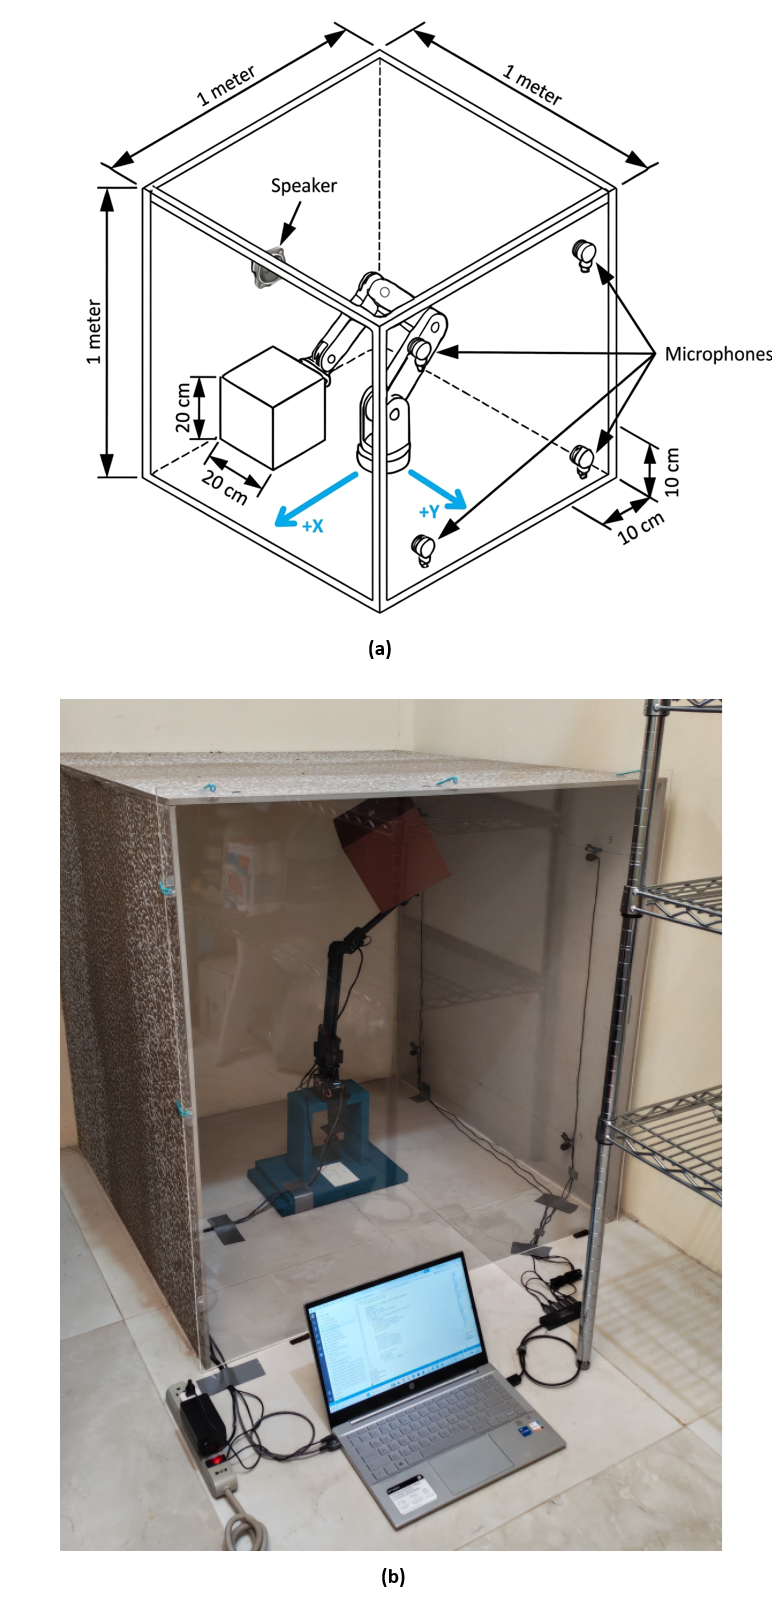
\includegraphics[height=15cm, width=8cm]{../img/Measuretogether.png}
            \caption{Measure box: (a) Conceptual sketch for the acoustic measurement box, and (b) actual implementation for the data acquisition task.}
        \label{mesurementbox}                         
        \end{center}
\end{figure}



\section{The Audio-Location Dataset for Model Training and Testing}

The dataset was collected through twenty‑six recording sessions. In each session, the robotic arm maintained a fixed angular value at its base and raised the cube to specific coordinates and orientations. The initial orientation of the cube was set with its sides parallel to the measurement box walls. The variables modified during each measurement were the cube’s location and orientation. For each location, nine different orientations were recorded. After completing these nine measurements, the robotic arm lowered the cube by decreasing its position along the Z axis, and the recording process was repeated for the new location. This procedure continued until the cube reached the bottom of the measurement box.

Audio from four channels was recorded. The acoustic signal was emitted four times, and the response was captured one microphone at a time. Each recording session consisted of 270 recordings, each containing four channels. A change of 10 degrees in the base of the robotic arm differentiated each recording session, producing a cylindrical envelope for the measurement area.

The coordinates of each measurement, obtained from the robotic arm, are shown in Fig. \ref{xyzlocations}. The distribution of points is presented in the plot, each blue column in the three dimensions corresponds to the points in a recording session, and each point containts the nine orientations captured at that location. The total number of sessions was limited by the rotational constraint of the robotic arm’s base, which allowed only 270 degrees of angular movement in its base. In total, 26 sessions were conducted, resulting in a dataset of 7020 recordings. 

\begin{figure}[!htb]
        \begin{center}        
            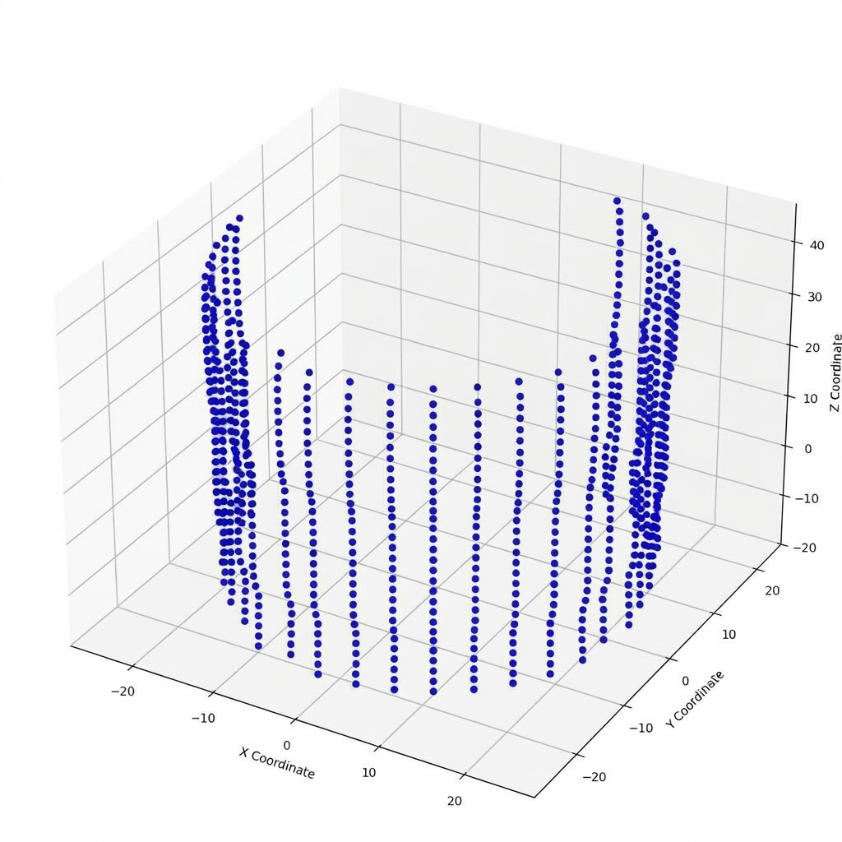
\includegraphics[height=12cm, width=12cm]{../img/allpoints.png}
            \caption{Scatter plot of cube locations for each recording in the dataset, the blue columns represent the 26 sessions, and each point in the column represents the nine orientations captured at that location.}
        \label{xyzlocations}                         
        \end{center}
\end{figure}

%##############################################################

The source audio signal was obtained by arbitrarily extracting a 0.3‑second segment from an acoustic melody. The spectrum of the signal has a bandwidth that reaches 10 kHz, with higher‑magnitude components concentrated at low frequencies. Before reproducing the source signal, the recording process is initialized by opening the capture window for one second. This procedure is repeated four times, once for each microphone. After completing the four recordings, the cube is moved to a new orientation until it complete the nine possible and after this it moves to a new location.



\section{The Audio-Location Processing Pipeline}


In figure \ref{fig:method} can be observed the processing pipeline for the acoustics signals. From the measurement box, the microphone array records four signals to output four audio channels, these channels are used to feed the pipelines. First in AudAlign step the audio signals are aligned due to the temporal unpredictability in the recording start time caused by the OS process scheduler, the signals from the four channels are aligned by exploiting the fact that the distance from the source to each microphone is identical. Therefore, the magnitude of the direct sound can be used as an alignment reference for the signals. In the same step, a signal‑integrity validation is performed in which each recording is divided into its main body and tail ( reverberation segment ), from the main segment, the signal power is computed, and from the tail, its duration is extracted. Signals whose power and tail length fall within predefined limits are considered valid and included in the dataset. The resulting dataset is used in four diferent scenarios, two of them use a CNN-based pipeline and the other two use an ESN-based pipeline. The CNN-based require the time series data to be transformed into an image representation, while the ESN-based pipelines learn from an audio to spectral sequence series transformation. Additionally, a beamforming approach is suggested to address the superposition creating a segmented origin representation of the acoustic reverberation, dividing the room space into four different regions. The sound originating from these regions is contained in a group of newly created channels that will also feed both CNN and ESN estimators.


\begin{figure}[hbt!]
	\begin{center}
		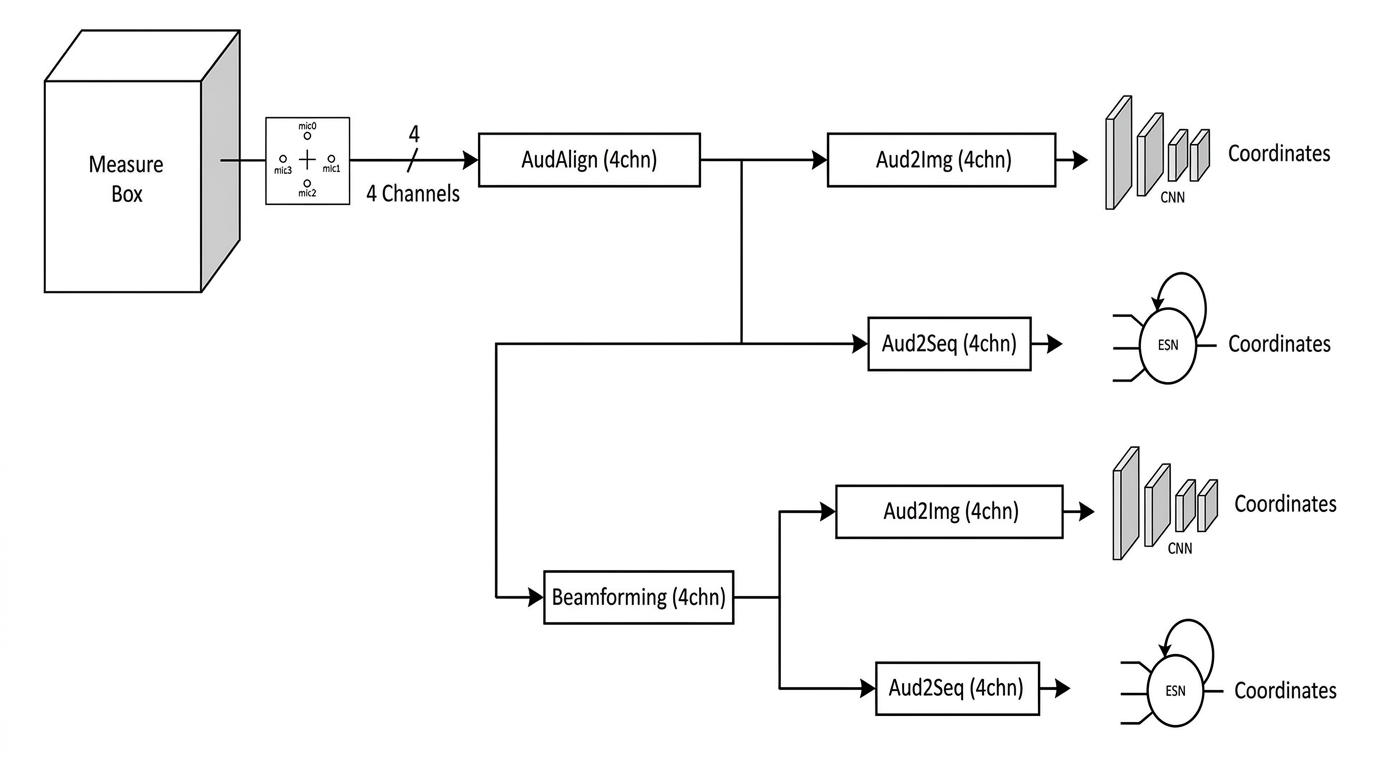
\includegraphics[width=16cm, height=8cm]{../img/AcousticPipeline.jpeg}
		\caption{Acoustic to location processing pipeline}
		\label{fig:method}
	\end{center}
\end{figure}


\section{Factors and Levels}

Factors are the independent variables that are going to be manipulated in the experiment, while levels are the different values that each factor can take. The factors and levels are selected based on the experimental design and the research questions being addressed. In this experiment, the factors include beamforming and network topology. Each factor has specific levels that will be tested to evaluate their impact in the task of estimating the location and orientation of the cube in the room. 

For the experimental analysis, the factors and their respective levels to consider are summarized in the table \ref{tab:facandlev}. The network factor has two levels, The CNN 
is the reference model, the one that will be used as a baseline for comparison considering that once the audio signals are transformed into an image representation, the CNN is a well-established model for image processing tasks becoming a good candidate for the task of estimating the location and orientation of the cube in the room, the other level of the network factor is the ESN, which is an memory and training efficient model that will be evaluated against the CNN. Also a beamforming factor is considered, which has two levels, with and without beamforming. The combination of these factors and levels will allow for a comprehensive evaluation of the performance of the different processing pipelines in estimating the location and orientation of the cube in the room. 

\begin{table}[hbt!]
	\caption{Factors and levels for the experiment.}
	\label{tab:facandlev}
	\begin{center}
		\begin{tabular}{|l|l|l|}
			\cline{2-3}
			\multicolumn{1}{c|}{}	& \multicolumn{2}{c|}{Factors} \\ 
			\cline{2-3}
			\multicolumn{1}{c|}{}	& Network &  Beamforming \\ \hline
			Levels
			& CNN     &    With  \\
			& ESN     &    Without  \\\hline
		\end{tabular}
	\end{center}
\end{table}


\section{Response Variables}

The networks in this research are configured as regression models, the outputs are the predicted coordinates (X, Y, Z) and orientation of the cube in the room. The response variables are the error between the predicted and actual values of these outputs, which are calculated as mean of the absolute difference between the predicted and actual values as shows in equation \ref{eq:mae}. The Mean Absolute Error (MAE) is used as the performance metric for evaluating the models. "The MAE is a widely used metric for regression tasks, as it provides a clear measure of the average magnitude of errors in predictions, without considering their direction. Lower MAE values indicate better model performance, as they reflect smaller discrepancies between predicted and actual values".


\begin{equation}
\label{eq:mae}
\text{MAE} = \frac{1}{n} \sum_{i=1}^{n} |y_i - \hat{y}_i|
\end{equation}



\section{Data Recollection for Model Evaluation}

To evaluate the performance of the models, a five-fold cross-validation approach are used. In this approach, the dataset is divided into five subsets, and the model is trained and tested five times, each time using a different subset as the test set and the remaining subsets as the training set. This process allows for a more robust evaluation of the model's performance and helps to mitigate any potential bias that may arise from using a single train-test split. The total 7020 samples are divided into five folds, with each fold containing near to 1,404 samples (A 80:20 ratio). The performance of the model is evaluated considering the Mean Absolute Error (MAE). The structure of the five-fold cross-validation and the corresponding performance metrics are summarized in Table \ref{tab:kfold_structure}. Due to the factor and levels we have 4 model variation to consider, and for each model variation the coordinates X, Y, Z, and orientation are evaluated, resulting in a total of 20 MAE to obtain for evaluation.

\begin{table}[h]
\centering
\begin{tabular}{lccc}
\hline
\textbf{Fold Iteration} & \textbf{Training Set} & \textbf{Test Set} & \textbf{Performance Metric} \\
\hline
Fold 1 & Fold 2, Fold 3, Fold 4, Fold 5 & Fold 1 & MAE$_1$ \\
Fold 2 & Fold 1, Fold 3, Fold 4, Fold 5 & Fold 2 & MAE$_2$ \\
Fold 3 & Fold 1, Fold 2, Fold 4, Fold 5 & Fold 3 & MAE$_3$ \\
Fold 4 & Fold 1, Fold 2, Fold 3, Fold 5 & Fold 4 & MAE$_4$ \\
Fold 5 & Fold 1, Fold 2, Fold 3, Fold 4 & Fold 5 & MAE$_5$ \\
\hline
\end{tabular}
\caption{Five-fold cross-validation structure and performance summary.}
\label{tab:kfold_structure}
\end{table}


\section{Statistical Tool Used for hipotesis Testing}

The groups of MAE obtained from the five-fold cross-validation for each model variation are considered as dependent samples because the same fold split of the dataset is used for each model evaluation. Two aproaches can be followed to evaluate the significance of the differences in the MAE between the different model variations. The first approach is to use a repeated measures ANOVA, which is a statistical test that compares means across multiple related groups. in order to use this approach, the assumptions of normality and sphericity must be met. If these assumptions are not met, a non-parametric alternative such as the Friedman test can be used. The Friedman test is a non-parametric test that compares the ranks of the data across multiple related groups. It does not assume normality and is suitable for small sample sizes. In the present work The Friedman test is used as the recomended option to determine if there are significant statistical differences in the MAE between machine learning models \cite{friedmanrecomendation}. 

In the friedman test, Instead of comparing the means of the groups, the Friedman test ranks the data within each fold. The ranks are then summed for each model variation, and the test statistic is calculated based on these rank sums. Finally The resulting values are compared to a chi-square distribution to find the p-value, which indicates the probability of observing the data if the null hypothesis is true \cite{friedmanprocess}.

The hypotheses for the test are as follows:
$H_0$: All models perform equally.
$H_1$: At least one model's performance is significantly different.

If the $p-value < 0.05$, reject $H_0$ and a post-hoc analysis is required to determine which specific models differ from each other.







